\chapter{Requirements and design} \label{chap:reqs}

The following section presents the identified objectives and the methodology we follow for the rest of the work.
We discuss the steps we have taken to analyse the existing QUIC and MQTT implementations to motivate our choice of libraries.
Additionally, we describe the test bench created for the network tests of the implementation and the methodology for its binary analysis.



\section{Requirements}

In order to create analyse QUIC as a transport layer protocol for IoT, we have identified the following requirements using a MoSCoW style analysis:

\begin{itemize}
    \item Must:
    \begin{itemize}
        \item We \textbf{must} create a test case for MQTT using QUIC - MQuicTT.
        \item We \textbf{must} analyse the performance of MQuicTT compared to base MQTT implementations.
        \item We \textbf{must} focus on realistic testing scenarios for evaluation.
    \end{itemize}
    \item Should:
    \begin{itemize}
        \item We \textbf{should} analyse a general methodology for reducing the hardware footprint of transport layer protocols for IoT.
        \item We \textbf{should} analyse the hardware footprint and feature set of TLS.
    \end{itemize}
    \item Could:
    \begin{itemize}
        \item We \textbf{could} create a QUIC extension that uses a lightweight security protocol.
    \end{itemize}
\end{itemize}

From these requirements, we have split the project into the following objectives:

\begin{itemize}
    \item \textbf{O1}: Compare existing QUIC and MQTT implementations that can act as underlying libraries.
    \item \textbf{O2}: Create an abstraction layer for the QUIC specific logic.
    \item \textbf{O3}: Implement MQuicTT by changing the underlying MQTT implementation to use this abstraction layer.
    \item \textbf{O4}: Create a test bench for the network performance analysis of MQuicTT.
    \item \textbf{O5}: Devise a methodology for trimming down the QUIC stack in terms of binary size.
    \item \textbf{O6}: Analyse the components of the MQuicTT binary.
    \item \textbf{O7}: Analyse the features of TLS and possible alternatives.
\end{itemize}

Hence, the rest of this chapter is split into sections corresponding to the design for each objective.

\section{Design of implementation}

In this section, we present a comparison of existing QUIC and MQTT implementations that can be used as underlying libraries for MQuicTT.Additionally, we discuss the high-level design of MQuicTT and the approach we have taken when it comes to using existing libraries compared to creating new protocol implementations.


\subsection{QUIC} \label{section:quic_impl}

We now compare the existing implementations of the QUIC protocol in the context of usability for IoT devices and present the reasoning behind our choice of QUIC library.
We have considered the mainstream implementations in the C, C++, Rust and Go programming languages as these are the languages that can be considered systems languages and would thus be the most widely used ones for IoT devices.
In addition to this, we did not consider implementations paired with a browser web engine as these would be impossible to use on hardware constrained devices.
Hence, we did not include notable implementations such as the QUIC implementation of the chromium web engine~\citep{chromium_quic_2021} and $Neqo$~\citep{mozilla_neqo_2022}.

Importantly, to analyse the performance of underlying QUIC implementations, we have transferred the same file using each implementation several times and have taken the average time to do so.
We repeated this while altering parameters as described in Section~\ref{chap:net_sim}.
The differences in transfer time were negligible and have hence not been presented as part of the comparison of libraries.
Hence, we compare QUIC implementations in terms of their TLS use, programming language and the binary size produced by their client and server implementations.

First, we consider the general landscape of available QUIC implementations to contextualise the ones developed in Rust.
Table~\ref{tab:quics} demonstrates the analysed QUIC implementations.
In order to find the size of the binary, we have used the Linux $ls$ utility.
In the case of the $mvfst$ implementation, we have taken further steps due to the reported binary size being far too large.
Therefore, we had to remove the C++ debug symbols that were causing the binary size to be over 300 MiB.
We have identified the following main methods by which QUIC implementations incorporate TLS:

\begin{itemize}
    \item Use of an external library - the implementation uses an external TLS API either by using a package manager in the case of Rust or by relying on an installed implementation in the case of C and C++.
    \item Use of own implementation - the implementation packages its implementation of the TLS protocol alongside QUIC.
\end{itemize}

This different use of TLS presented a challenge in calculating the binary size of the QUIC servers and clients.

\begin{table}[ht]
    \caption{The identified QUIC implementations and their binary size footprint. The footprint has been split into a client and server footprint using a minimal reproducible example for each. We used each implementation to create an example client and server capable of sending and receiving QUIC packets and analysed the binary size. Where provided, we compared this to the given examples to ensure as little implementation bias as possible. However, this is still not a perfect estimate, and some variance due to implementation details may be present.}\label{tab:quics}
    %\tt 
    \rowcolors{2}{}{gray!3}
    \begin{tabular}{@{}lllll@{}}
        \toprule
        \textbf{Implementation} & \textbf{PL}   & \textbf{Footprint (client) (MiB)} & \textbf{Footprint (server) (MiB)} & \textbf{TLS method} \\
        ngtcp2                  & \texttt{C}    & \texttt{3.4}                      & \texttt{4.3}                      & \texttt{External}   \\
        picoquic                & \texttt{C}    & \texttt{3.2}                      & \texttt{3.9}                      & \texttt{External}   \\
        msquic                  & \texttt{C}    & \texttt{3.2}                      & \texttt{4.1}                      & \texttt{External}   \\
        quic-go                 & \texttt{Go}   & \texttt{8.7}                      & \texttt{9.9}                      & \texttt{External}   \\
        Quinn                   & \texttt{Rust} & \texttt{9.1}                      & \texttt{9.5}                      & \texttt{External}   \\
        Quiche                  & \texttt{Rust} & \texttt{7.8}                      & \texttt{7.0}                      & \texttt{Own}        \\
        mvfst                   & \texttt{C++}  & \texttt{11.1}                     & \texttt{12.0}                     & \texttt{Own}        \\
        \bottomrule
    \end{tabular}
\end{table}

Specifically, in each case, we have considered the external dependencies that a developer will have to install to run the QUIC implementation on a device.
Hence, in the case of C implementations that require an external TLS library, such as OpenSSL, to be installed and linked on the system, we have opted to add the binary size produced by OpenSSL to the size of the QUIC binaries.
Additionally, in the case of $picoquic$, we have added the size of the $picotls$ dependency on top of the size of OpenSSL.

\begin{figure}[ht]
    \centering
    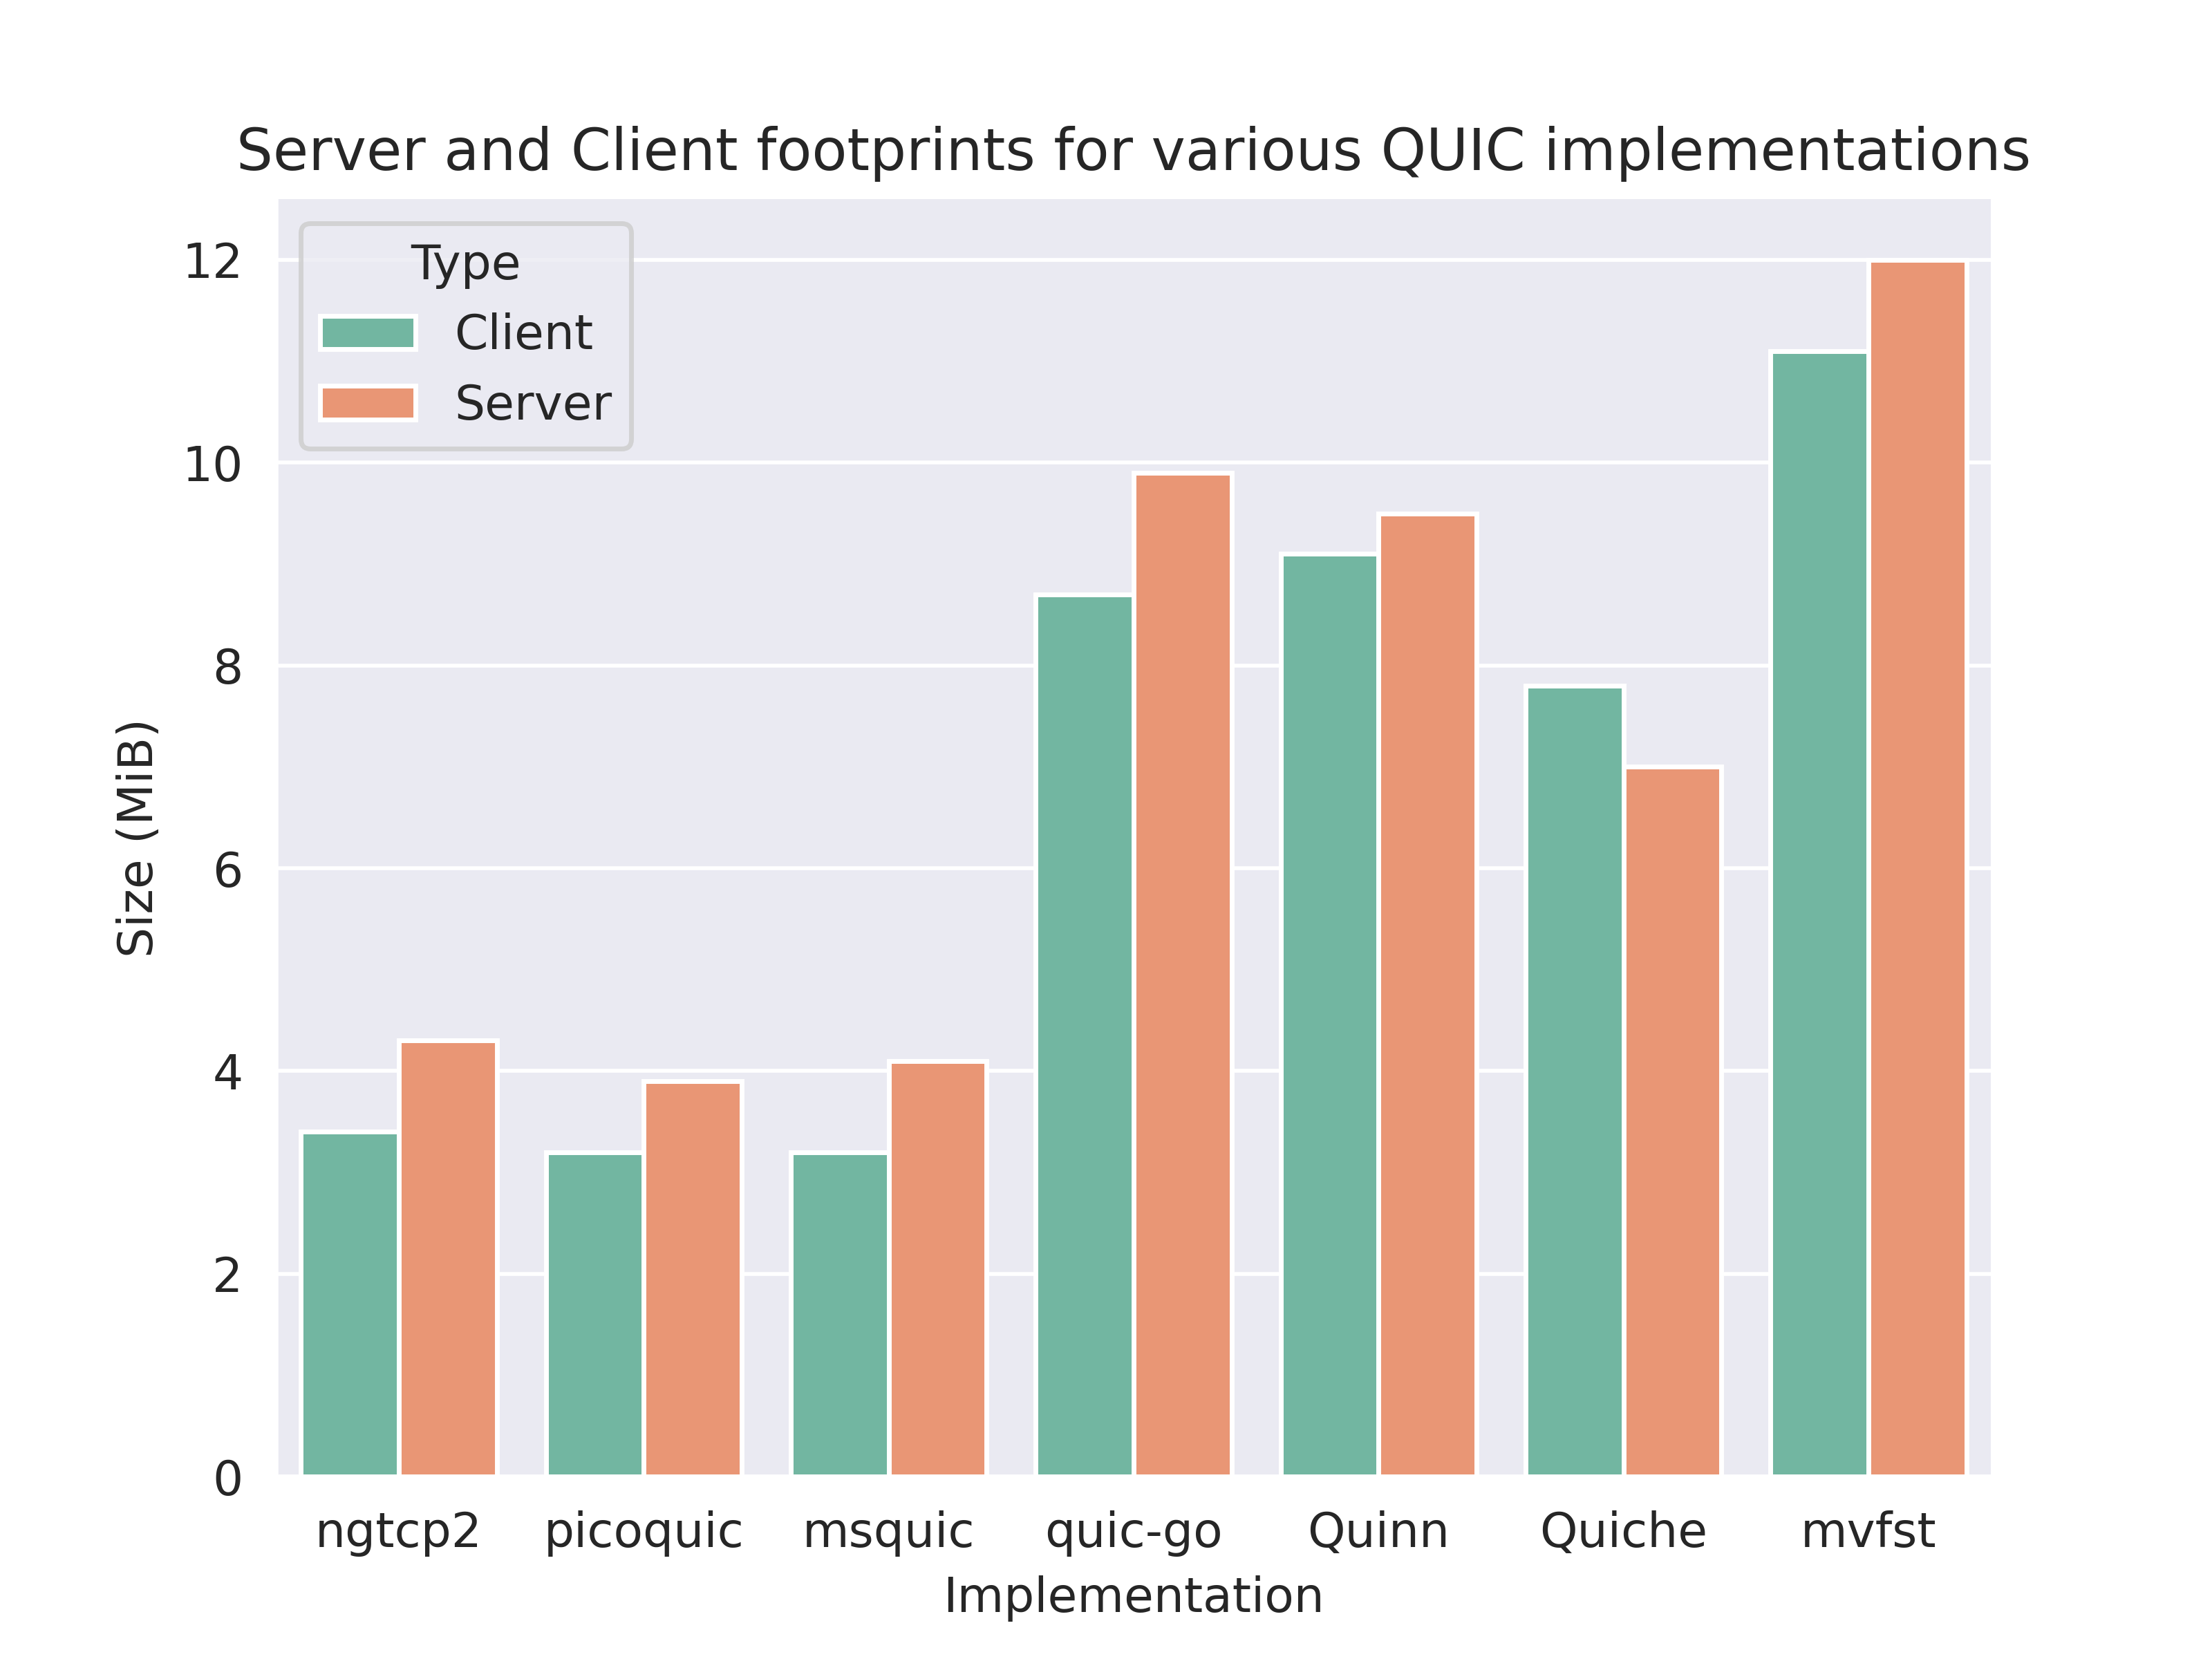
\includegraphics[width=1\linewidth]{images/quic_impls.png}
    \caption{The sizes of the client and server footprints for the selected QUIC implementations. Notable, only Quiche produced a server binary with a smaller size than its corresponding client binary. It is hard to estimate the error margin for the data as this depends on implementation details in the example client and servers.}
    \label{fig:quic_impls}
\end{figure}

Figure~\ref{fig:quic_impls} further visualises the comparison of binary sizes between the various implementations.
This is an important aspect due to the aforementioned hardware constraints.
Notably, we can see that five out of the seven analysed implementations opt to use an external TLS library or engine.
Out of these five, all C implementations supported OpenSSL, with the Go and Rust implementations opting to use a TLS library.
In the case of $quic-go$, this was the $crypto/tls$ package, and in the case of Rust, $rustls$.
We can also see that the Rust implementations are not drastically different in binary footprint size.

Notably, although Go is described as memory safe, it does not opt for compile-time memory safety and instead uses the panic model.
The panic model is another advantage of Rust compared to languages such as Go, as Rust provides these guarantees using a robust type system.
Between the two Rust implementations - Quinn and Quiche, we chose Quinn due to issues with the Quiche library.
On the other hand, Quiche opts to make the user create a $mio$ event loop, which interfered with the $tokio$ runtime environment used in our chosen MQTT implementation discussed in the next section.
In addition to this, we found that the Quinn API is easier to work with when creating the intermediate library discussed in Chapter~\ref{chapter:quic_socket}; for example, Quinn handles the QUIC handshake in the library and does not require the developer to create an event loop.

\section{MQTT}\label{section:mqtt_impls}

Compared to QUIC, the choice of MQTT implementation was substantially simpler.
The criteria for MQTT implementation were that it was developed in Rust, implemented both a client and a broker, had widespread use and adhered to MQTT version 5.0.
Based on the above criteria we identified two possible implementations:\citepos{eclipse_eclipse_2018} $paho$ and $rumqtt$~\citep{bytebeam_rumqtt_2020}.
We opted to use $rumqtt$ at it is a native Rust implementation, whereas $paho$ provides a rust binding to an underlying C implementation.
We chose to evaluate a fully Rust native MQTT/QUIC stack as this provides an opportunity for a valuable comparison to mainstream C implementations.
Other available implementations supported only one side of the MQTT protocol or only supported version 3.1.1.

$Rumqtt$ provides to components for an MQTT application - $rumqttc$ and $rumqttd$.
The former can be used to create an MQTT client, and the latter a broker.
However, the code base for these is somewhat similar, easing the incorporation of QUIC.
Both components provide an interface for supporting asynchronous communication using a $tokio$ runtime, which fits nicely into our choice of QUIC implementation as $Quinn$ requires a $tokio$ environment.
By default, $rumqtt$ uses TCP as its transport layer protocol and TLS through $rustls$.
All underlying implementation assumptions remain equal because this is the same library as $Quinn$ uses.


\subsection{MQuicTT design}

To create MQuicTT, we have, as previously seen, opted to use existing implementations of QUIC and MQTT.
An alternate approach to this would be creating implementations from scratch that could be optimised for our use case.
However, we demonstrate an actual use case by opting to use existing libraries.
These libraries have both been built for production use and are relatively widely deployed.
Hence, we are more likely to get accurate results.
In addition to this, the development time needed to create implementations for these protocols from scratch would far exceed this project's scope.

However, we have created an intermediate library that will act as an abstraction from the QUIC logic - $QuicSocket$.
By creating this intermediate library and ensuring that its API mimics a standard TCP socket, we lower the difficulty of porting $rumqtt$ to QUIC.
Additionally, this library can be used for any application that uses the QUIC protocol.

Hence, the design for the implementation has been split into two broad stages.
In the first stage, we create an abstraction around $quinn$ that acts as a socket for the QUIC protocol.
In the second stage we use the resulting socket library to port $rumqtt$ to QUIC.

Further discussion of specific technical choices that we have made during the implementation can be found in Chapter~\ref{chap:impl}.

\section{Network performance experiment design} \label{chap:net_sim}

We now discuss the analysis methodology for the performance portion of the implementation evaluation.
That is, this section focuses on evaluating MQuicTT against the base $rumqtt$ implementation.

The critical consideration for this design is the scenarios in which IoT devices are used.
When evaluating the network performance of the implementations, we considered two options: using real IoT devices or using a network simulation tool.
Due to technical limitations that came with using real devices, such as not being able to access the router of our network, we opted for simulation.
In this section, we will discuss how we used Mininet~\citep{lantz_mininet_2021}, a realistic virtual network, in our evaluation.

Mininet is a tool that network developers and researchers can use to create software-defined networks (SNDs) using the $OpenFlow$ standard.

\begin{figure}[ht]
    \centering
    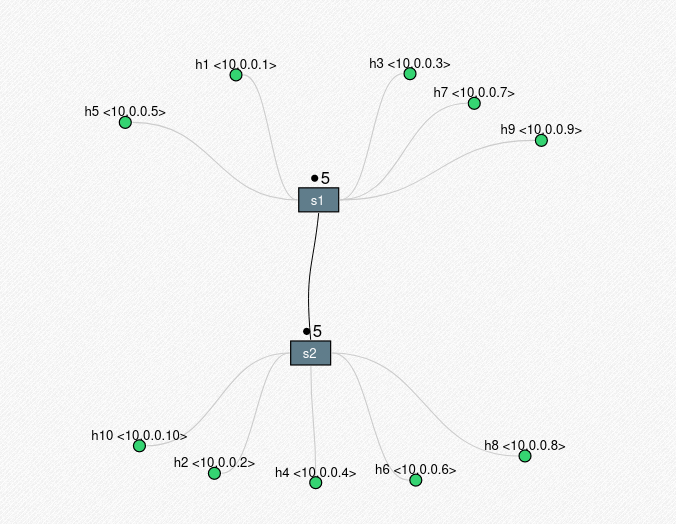
\includegraphics[width=0.9\linewidth]{images/mininet_topo.png}
    \caption{The resulting Dumbbell topology with the broker being h9 - the central node. The link between the central switch and the central host results in a congested network.}
    \label{fig:mininet-topo}
\end{figure}

Using the Python API provided, we created the network topology shown in Figure~\ref{fig:mininet-topo}.
The script takes several parameters to create the following three scenarios:

\begin{itemize}
    \item A synthetic scenario testing the limits of implementations.
    \item A realistic scenario based on a smart-home use-case.
    \item A realistic scenario based on a 3D printer farm.
\end{itemize}

The topology for all three scenarios remains the same - a minimum spanning tree of a typical IoT mesh network.
When designing this topology, we needed it to reflect various realistic IoT scenarios.
We can imagine this as a singular room in a home with all of its smart appliances being a cluster in the smart home or a cluster of 3D printers in a section of a farm in the 3D printer farm.
The critical feature of this topology is that many clusters are connected to a central broker that controls the topology, hence creating a dumbbell structure.
The full definition of this topology can be found in Appendix~\ref{appendix:topo}.
The variables that the script changes between scenarios and simulations are the link's \textit{bandwidth}, \textit{delay} and the rate of \textit{packet loss}.

The bandwidth of a link is the maximum rate of data transfer we can achieve.
In contrast to bandwidth in signal processing, we measure bandwidth in bits per second rather than hertz in computer networking.
The delay of a link specifies the latency of the link.
It is the time that a bit of data takes to travel across a link. 
We measure this in milliseconds.
Link delay corresponds to the geographical distance between the communicating parties; however, in the case of IoT, we can expect devices to be in local proximity.
Lastly, the packet loss rate shows the percentage of corrupted or dropped packets in transit.
Various protocols having to retransmit packets also adds to the delay of data transfer.
Importantly, we have only considered the typical circumstances of packet loss and have not included scenarios such as interference or packet loss attacks.

The bandwidth and delay numbers correspond, as closely as possible, to various link types in a network.
To do so, for the smart-home scenario, we have gathered data from the~\cite{ofcom_uk_2021} report on UK broadband speeds.
There were specific cases in which it was not possible to find this data in the report; hence it was augmented using a similar methodology in work conducted by~\cite{previdi_is-is_2019} and in the case of ZigBee, the work by~\citet{alena_fault_2011}.

\begin{table}[ht]
    \caption{The parameters chosen for each link simulation in Mininet in the smart home scenario. The types of links were chosen as the most commonly occurring ones in IoT use cases.}\label{tab:links:home}
    %\tt 
    \rowcolors{2}{}{gray!3}
    \begin{tabular}{@{}llll@{}}
        \toprule
        \textbf{Simulated Link Type} & \textbf{Link bandwidth (Mb/s)} & \textbf{Link delay (ms)} & \textbf{Packet loss rate (\%)} \\
        Wi-Fi                        & \texttt{30}                    & \texttt{10}              & \texttt{2}                     \\
        ZigBee                       & \texttt{0.25}                  & \texttt{5}               & \texttt{1}                     \\
        4G                           & \texttt{4}                     & \texttt{20}              & \texttt{1.5}                   \\
        3G                           & \texttt{1}                     & \texttt{40}              & \texttt{1.5}                   \\
        100Mb Ethernet               & \texttt{100}                   & \texttt{1}               & \texttt{0.2}                   \\
        \bottomrule
    \end{tabular}
\end{table}

Hence, we expect that the bandwidth and link delay numbers accurately represent a real-world scenario.
However, it was complicated to find exact estimates for packet loss rates, with most sources describing approximations for a stable connection~\citep{sdu_ictp-sdu_2013} and not precise measurements.
Hence, the data are best estimates, cross-validated through the different sources and are not exact values.

In the case of the smart home scenario, as presented in Table~\ref{tab:links:home}, we expect that our packet loss rates are accurate as these, as previously stated, do appear in the home broadband reports and other studies.
In the case of the 3D printer, as presented in Table~\ref{tab:links:3d} farm scenario, due to the number of machines and the interference these cause in a 3D printer farm, we modelled this scenario to have more packet loss.
We specifically chose this scenario to test the benefits that QUIC should receive in an environment with high packet loss.
However, we found it difficult to find exact data on packet loss percentages in smart factories or workshops; hence, we expect a margin of error on some of the values.

In general, we can assume that the packet loss rates will increase by some constant factor across all links.
Hence, we have also created a synthetic scenario with extreme packet loss as presented in Table~\ref{tab:links:synth}.
If the protocol performs well for an extreme scenario, we can expect it to also perform well for packet loss percentages up to that scenario.

\begin{table}[ht]
    \caption{The parameters chosen for each link simulation in Mininet in the 3D printer farm scenario. The data assumes a typical IoT setup where most devices are within local geographical proximity. That is, the devices are communicating with each other within the range of one factory or site, with only the central node communicating with some server.}\label{tab:links:3d}
    %\tt 
    \rowcolors{2}{}{gray!3}
    \begin{tabular}{@{}llll@{}}
        \toprule
        \textbf{Simulated Link Type} & \textbf{Link bandwidth (Mb/s)} & \textbf{Link delay (ms)} & \textbf{Packet loss rate (\%)} \\
        Wi-Fi                        & \texttt{30}                    & \texttt{10}              & \texttt{5}                     \\
        ZigBee                       & \texttt{0.25}                  & \texttt{5}               & \texttt{3}                     \\
        4G                           & \texttt{4}                     & \texttt{20}              & \texttt{2.5}                   \\
        3G                           & \texttt{1}                     & \texttt{40}              & \texttt{2.5}                   \\
        100Mb Ethernet               & \texttt{100}                   & \texttt{1}               & \texttt{0.5}                   \\
        \bottomrule
    \end{tabular}
\end{table}

\begin{table}[ht]
    \caption{The parameters chosen for each link simulation in Mininet in the synthetic scenario. Here we opt for extreme packet loss scenarios to test the boundaries of the protocols. We opted for 20 times the normal packet loss that the link can expect in each case. We have also tested this for higher values however all protocol implementations greatly suffered in performance beyond this.}\label{tab:links:synth}
    %\tt 
    \rowcolors{2}{}{gray!3}
    \begin{tabular}{@{}llll@{}}
        \toprule
        \textbf{Simulated Link Type} & \textbf{Link bandwidth (Mb/s)} & \textbf{Link delay (ms)} & \textbf{Packet loss rate (\%)} \\
        Wi-Fi                        & \texttt{30}                    & \texttt{10}              & \texttt{15}                     \\
        ZigBee                       & \texttt{0.25}                  & \texttt{5}               & \texttt{15}                     \\
        4G                           & \texttt{4}                     & \texttt{20}              & \texttt{20}                   \\
        3G                           & \texttt{1}                     & \texttt{40}              & \texttt{20}                   \\
        100Mb Ethernet               & \texttt{100}                   & \texttt{1}               & \texttt{4}                   \\
        \bottomrule
    \end{tabular}
\end{table}

We evaluate MQuicTT's performance using the presented topologies and respective simulation parameters in the following way.
Each protocol transmits 100 messages from a client to a broker for each data link.

During this, we measure the following:

\begin{itemize}
    \item The time taken for the underlying transport protocol to establish a connection.
    \item The time taken to transmit the message to the broker.
\end{itemize}

This is repeated several times to ensure that variance does not affect results.
This process is repeated for all three testing scenarios.

In general, MQTT allows for messages with a maximum size of approximately 260MB.
However, this is a huge message, and most publicly deployed brokers reject it, so we created a representative message for each use case.
Each topic in MQTT consists of a hierarchy of topic levels separated by a forward slash.
For example, in a smart home scenario, we may have a topic like $home/groundfloor/kitchen/temp$ to control the temperature in the kitchen via a smart thermostat.
A topic may also include a wildcard.
The topic string $home/groundfloor/+/temp$ includes a \textit{single-level} wildcard that will match an arbitrary string.
This would match the topic $home/groundfloor/lounge/temp$, but not match the topic $home/secondfloor/kitchen/temp$.
If a client wishes to subscribe to multiple topics with the same prefix, a \textit{multi-level} wildcard may be used.
For example, the topic $home/secondfloor/kitchen/\#$ can be used to subscribe to all topics with a prefix matching the string before the hash character.
Notably, brokers reserve topics for system messages starting with the \$ character.

The chosen topic and the transmitted message for each scenario can be found in Appendix~\ref{appendix:mqtt_message}.
The messages were devised based on an arbitrary command that may be issued to an IoT device present in the scenario.
For the synthetic scenario we opted to use a message that is considerably longer, to test the limits of each implementation.
This message simply consisted of a paylaod with a field replicated thousands of times.
It has ben omitted from the Appendix due to being too long.

\section{Binary size experiment design}

The last section of this chapter describes how we have conducted further analysis on the binary size of the QUIC protocol that underlines MQuicTT.
The focus of this section is to see if the QUIC stack contributes a significant overhead to MQuicTT's binary size and how we can reduce this overhead.
We expect that the QUIC stack will contribute to the majority of the size of MQuicTT as MQTT itself is designed to have a low code size overhead.
Hence, the first step of this part of the analysis will be to determine how much QUIC contributes to the binary size.

In order to get a breakdown of the binary we have used the $cargo-bloat$~\footnote{cargo-bloat - \url{https://lib.rs/crates/cargo-bloat}} utility.
The utility analyses the binary using custom ELF, DWARF and Mach-O parsers and disassembles the binary to look for references and links to anonymous data.
Doing so creates a map of the binary that shows where every byte has a label attached to it.

This utility provides the composition of a Rust binary. 
However, it is not perfect and results in some margin of error.
Unfortunately, this margin of error is also not easily measurable.
By comparing the total size of the binary as reported by $cargo-bloat$ to the size reported by the operating system, we have deduced that the total error margin is within $1\%$ with good precision.
This should mean that we can get a somewhat accurate error margin on the components. 
However, it is also possible that the internal calculations are inaccurate despite the overall size being accurate.

The next step in this stage will be analysing methods for trimming down the QUIC stack binary size.
Hence, in this stage, we shift our focus to the binary produced by $QuicSocket$.
To reduce the binary size, we opt to use the method established by~\citet{eggert_towards_2020} as recreating these steps may show a general framework for reducing binary sizes for hardware constrained devices.
Notably, our application already handles client and server code separately; the MQTT broker requires a different binary to the MQTT client.

Hence, the steps we take are as follows:

\begin{itemize}
    \item Compile the binary for a 32-bit target by setting the $target$ flag in cargo to $i686-unknown-linux-gnu$.
    \item Remove any error handling code beyond what is needed for the binary to compile.
    \item Remove any code that writes to standard output.
\end{itemize}

After every step, we record the difference in binary size made by the change using the same methodology.
